% For LaTeX-Box: root = stat105_F15_exam1B.tex 
%%%%%%%%%%%%%%%%%%%%%%%%%%%%%%%%%%%%%%%%%%%%%%%%%%%%%%%%%%%%%%%%%%%%%%%%%%%%%%%%
%  File Name: stat105_F15_exam1B.tex
%  Purpose:
%
%  Creation Date: 24-09-2015
%  Last Modified: Tue May  3 08:29:28 2016
%  Created By:
%%%%%%%%%%%%%%%%%%%%%%%%%%%%%%%%%%%%%%%%%%%%%%%%%%%%%%%%%%%%%%%%%%%%%%%%%%%%%%%%
\documentclass[addpoints]{examsetup}\usepackage[]{graphicx}\usepackage[]{color}
%% maxwidth is the original width if it is less than linewidth
%% otherwise use linewidth (to make sure the graphics do not exceed the margin)
\makeatletter
\def\maxwidth{ %
  \ifdim\Gin@nat@width>\linewidth
    \linewidth
  \else
    \Gin@nat@width
  \fi
}
\makeatother

\definecolor{fgcolor}{rgb}{0.345, 0.345, 0.345}
\newcommand{\hlnum}[1]{\textcolor[rgb]{0.686,0.059,0.569}{#1}}%
\newcommand{\hlstr}[1]{\textcolor[rgb]{0.192,0.494,0.8}{#1}}%
\newcommand{\hlcom}[1]{\textcolor[rgb]{0.678,0.584,0.686}{\textit{#1}}}%
\newcommand{\hlopt}[1]{\textcolor[rgb]{0,0,0}{#1}}%
\newcommand{\hlstd}[1]{\textcolor[rgb]{0.345,0.345,0.345}{#1}}%
\newcommand{\hlkwa}[1]{\textcolor[rgb]{0.161,0.373,0.58}{\textbf{#1}}}%
\newcommand{\hlkwb}[1]{\textcolor[rgb]{0.69,0.353,0.396}{#1}}%
\newcommand{\hlkwc}[1]{\textcolor[rgb]{0.333,0.667,0.333}{#1}}%
\newcommand{\hlkwd}[1]{\textcolor[rgb]{0.737,0.353,0.396}{\textbf{#1}}}%

\usepackage{framed}
\makeatletter
\newenvironment{kframe}{%
 \def\at@end@of@kframe{}%
 \ifinner\ifhmode%
  \def\at@end@of@kframe{\end{minipage}}%
  \begin{minipage}{\columnwidth}%
 \fi\fi%
 \def\FrameCommand##1{\hskip\@totalleftmargin \hskip-\fboxsep
 \colorbox{shadecolor}{##1}\hskip-\fboxsep
     % There is no \\@totalrightmargin, so:
     \hskip-\linewidth \hskip-\@totalleftmargin \hskip\columnwidth}%
 \MakeFramed {\advance\hsize-\width
   \@totalleftmargin\z@ \linewidth\hsize
   \@setminipage}}%
 {\par\unskip\endMakeFramed%
 \at@end@of@kframe}
\makeatother

\definecolor{shadecolor}{rgb}{.97, .97, .97}
\definecolor{messagecolor}{rgb}{0, 0, 0}
\definecolor{warningcolor}{rgb}{1, 0, 1}
\definecolor{errorcolor}{rgb}{1, 0, 0}
\newenvironment{knitrout}{}{} % an empty environment to be redefined in TeX

\usepackage{alltt}

\usepackage{etoolbox}
\usepackage{tikz,pgfplots}
\usepackage{graphicx, fancyhdr}
\usepackage{amsmath, amsfonts}
\usepackage{color}

%% For LaTeX-Box: root = stat105_exam1_info.tex 
%%%%%%%%%%%%%%%%%%%%%%%%%%%%%%%%%%%%%%%%%%%%%%%%%%%%%%%%%%%%%%%%%%%%%%%%%%%%%%%%
%  File Name: stat105_exam1_info.tex
%  Purpose:
%
%  Creation Date: 24-09-2015
%  Last Modified: Thu Sep 24 13:51:36 2015
%  Created By:
%%%%%%%%%%%%%%%%%%%%%%%%%%%%%%%%%%%%%%%%%%%%%%%%%%%%%%%%%%%%%%%%%%%%%%%%%%%%%%%%
\newcommand{\course}[1]{\ifstrempty{#1}{STAT 105}{STAT 105, Section #1}}
\newcommand{\sectionNumber}{B}
\newcommand{\examDate}{October 1, 2015}
\newcommand{\semester}{FALL 2015}
\newcommand{\examNumber}{II}

\newcommand{\examTitle}{Exam \examNumber}

\runningheader{\course{\sectionNumber}}{Exam \examNumber}{\examDate}
\runningfooter{}{}{Page \thepage of \numpages}

\newcommand{\examCoverPage}{
   \begin{coverpages}
   \centering
   {\bfseries\scshape\Huge Exam I \par}
   \vspace{1cm}
   {\bfseries\scshape\LARGE \course{\sectionNumber} \par}
   {\bfseries\scshape\LARGE \semester \par}

   \vspace{2cm}

   \fbox{\fbox{\parbox{5.5in}{\centering 

      \vspace{.25cm} 
      
      {\bfseries\Large Instructions} \\

      \vspace{.5cm} 

      \begin{itemize}
         \item  The exam is scheduled for 80 minutes, from 8:00 to 9:20 AM. At 9:20 AM the exam will end.\\
         \item  A forumula sheet is attached to the end of the exam. Feel free to tear it off.\\
         \item  You may use a calculator during this exam.\\
         \item  Answer the questions in the space provided. If you run out of room, continue on the back of the page. \\
         \item  If you have any questions about, or need clarification on the meaning of an item on this exam, please ask your instructor. No other form of external help is permitted attempting to receive help or provide help to others will be considered cheating.\\
         \item  {\bfseries Do not cheat on this exam.} Academic integrity demands an honest and fair testing environment. Cheating will not be tolerated and will result in an immediate score of 0 on the exam and an incident report will be submitted to the dean's office.\\
      \end{itemize}

   }}}

   \vspace{2cm}

   \makebox[0.6\textwidth]{Name:\enspace\hrulefill}

   \vspace{1cm}

   \makebox[0.6\textwidth]{Student ID:\enspace\hrulefill}
   \end{coverpages}

}


\newcommand{\course}[1]{\ifstrempty{#1}{STAT 105}{STAT 105, Section #1}}
\newcommand{\sectionNumber}{A}
\newcommand{\examDate}{May 3, 2016}
\newcommand{\semester}{Spring 2016}
\newcommand{\examNumber}{III}

%%%%%%%%%%%%%%%%%%%%%%%%%%%%%%%%%%%%%%%%%%%%%%%%%%%%%%%%%%%%%%%%%%%%%%%%%%%%%%%%
\IfFileExists{upquote.sty}{\usepackage{upquote}}{}
\begin{document}

%-- : R code (Code in Document)



\examCoverPage

\begin{questions}

\question[2]
(TRUE/FALSE) A random sample of 1000 student's Statistics exam scores was drawn from the population of all possible Stat scores (an unknown distribution).
Once the sample mean is computed, it can be viewed as the distribution/population mean.

\vspace{1cm}

\question[2]
(TRUE/FALSE) While trying to figure out the probability that the sample mean for a data of size 10 would exceed a value, we can apply the central limit theorem.

\vspace{1cm}

\question

%-- question1: R code (Code in Document)


A pH meter is a tool used to determine the acidity of a liquid. 
During calibration, the repeated measures are taken on two different liquids, one with a known pH of 3 and the other with a known pH of 11.

\begin{itemize}

   \item Readings with pH = 11: $ 11.5, 11.3, 11.3, 11.4, 11.4, 11.4, 11.5, 11.5 $ \\

   \item Readings with pH = 3: $ 3.1, 2.9, 3.2, 3.1, 2.7, 3.4, 3.1, 2.8 $ \\

\end{itemize}


\begin{parts}
   \part[2] At what pH is the meter more accurate?

   \vspace{1cm}

   \part[2] At what pH is the meter more precise?

   \vspace{1cm}

\end{parts}

\vspace{1cm}

\question 
%-- functionsAndDatasets: R code (Code in Document)

A sample of size 5 was drawn from a population and the resulting observations are reported below. 
$$
   2.2, 2, 2.4, 2.4, 2, 10.3
$$
Using these observed values, report the following:

\vspace{0.5cm}

\begin{parts}

   \part[2] the mean  
   \vspace{1.5cm}

   \part[2] the median
   \vspace{1.5cm}

   \part[2] the variance 
   \vspace{2cm}

   \part[2] the standard deviation 
   \vspace{1.5cm}

\end{parts}

\newpage

\question
Portable pneumatic pumps have long been used by hobby machinists, but are gaining renewed interest as robotics are becoming a more common part of our daily lives.
Specifically, drones can make use of such pumps due to their weight benefits over hydraulic pumps with equivalent strength.
Amazon is experimenting with using such pumps in its delivery drones and is interested in factors effecting the lifetime of the pumps.

A team of engineers working for Amazon has been tasked with developing pumps for delivery drones that improve both time-in-flight (measured in hours) and the number of pump-actions (the number of times the drone uses the pump).
With those goals in mind, the team designed three pumps: a single-piston/single-stage design, a dual-piston/single-stage design, and a dual-piston/dual-stage design.
The engineers are testing the pumps with three types of compressed gas: OFN (oxygen-free nitrogen), Carbon dioxide, and Oxygen.
Concerned about environmental effects, the engineers selected four locations to test the drones in - San Antonio, Seattle, Lexington, and Amherst in which to test the drones.

In all four locations they tested the every design-gas combination in five drones (45 drones in each location).
The drones delivered 5 pound packages from an initial location to a location 2000 meters away, retrieved the package, and returned it to the original point.
The number of deliveries and the flight time were recorded for each drone.

Note: \((\text{3 designs}) \cdot (\text{3 gas types}) \cdot (\text{5 drones}) \cdot (\text{4 locations}) = \text{180 total drones}\)

The goal is to determine is to identify how to maximize both flight time and number of deliveries.

\begin{parts}
   \part[2] Is this an experiment or an observational study? Explain.

  \vspace{2cm}

  \part Identify each of the following and describe them as numeric (in which case, identify whether it is continuous or discrete) or categorcial (in which case list the possible levels).

  \vspace{1cm}

   \begin{subparts}
      \subpart[2] Identify the response variable(s):

      \vspace{2cm}

      \subpart[2] Identify the experimental variable(s):

      \vspace{2cm}

      \subpart[2] Blocking variable(s):

      \vspace{2cm}

   \end{subparts}

   \part[2] Identify two controlled variables used in this process.

   \vspace{2cm}

\end{parts}

\pagebreak

\question[12] 
The data reported below are the times to failure (in millions of cycles) of high-speed turbine engine bearings made out of two different compounds.

%-- compounds: R code (Code in Document)
% latex table generated in R 3.2.4 by xtable 1.8-2 package
% Tue May  3 08:29:30 2016
\begin{table}[ht]
\centering
\begin{tabular}{lrrrrrrrrrr}
  \hline
  & \multicolumn{10}{c}{Bearing Number} \\
  & 1 & 2 & 3 & 4 & 5 & 6 & 7 & 8 & 9 & 10 \\
 \hline
Compound 1 & 3.03 & 5.53 & 5.60 & 9.30 & 9.92 & 12.51 & 12.95 & 15.21 & 16.04 & 16.84 \\ 
  Compound 2 & 3.19 & 4.26 & 4.47 & 4.53 & 4.67 & 4.69 & 5.78 & 6.79 & 9.37 & 12.75 \\ 
   \hline
\end{tabular}
\end{table}


For Compound 1, the first quartile is 5.6, the median is is 11.215 and the interquartile range is 9.61.

For Compound 2, the first quartile is 4.47, the median is is 4.68 and the interquartile range is 2.32.

\vspace{0.5cm}

Using the axes below, create a box plot for \textbf{time to failure} of each compound.

\begin{itemize}
   \item Label the values of the boundaries of the boxes
   \item Label the values the ends of the upper and lower whiskers
   \item Draw a star over unusual observations.
\end{itemize}

\textit{For any partial credit, show all work in the additional space}

\vspace{1cm}

%-- : R plot (results in document)
\begin{knitrout}
\definecolor{shadecolor}{rgb}{0.969, 0.969, 0.969}\color{fgcolor}
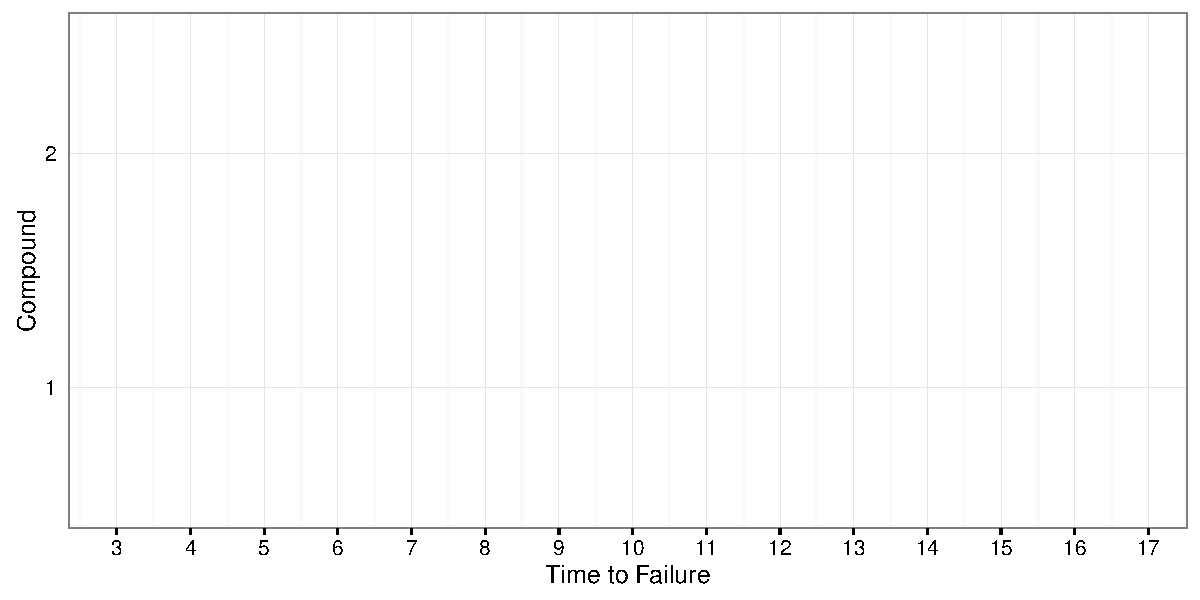
\includegraphics[width=.9\linewidth]{figure/unnamed-chunk-2-1} 

\end{knitrout}
\pagebreak

\question

%-- : R code (Code in Document)


The quality of a diamond is often described in terms of the four C's:
carat (the diamonds mass, with 1 carat = 200 milligrams), 
cut (a description of how well the diamond has been shaped),
color (the less color the more rare),
clarity (a description of the flaws in the diamond).
Of these, carat is the most easily understood in terms of its impact on the diamonds value: 
all things being equal, the larger the diamond the higher its value.

The following plot shows the sale price of 375 diamonds (in thousands of dollars), which were appraised by experts as having an ideal cut, internally flawless clarity, and being colorless or essentially colorless.

%-- : R figure (code in document - set include=FALSE to remove)

\begin{knitrout}
\definecolor{shadecolor}{rgb}{0.969, 0.969, 0.969}\color{fgcolor}\begin{figure}[h]

{\centering 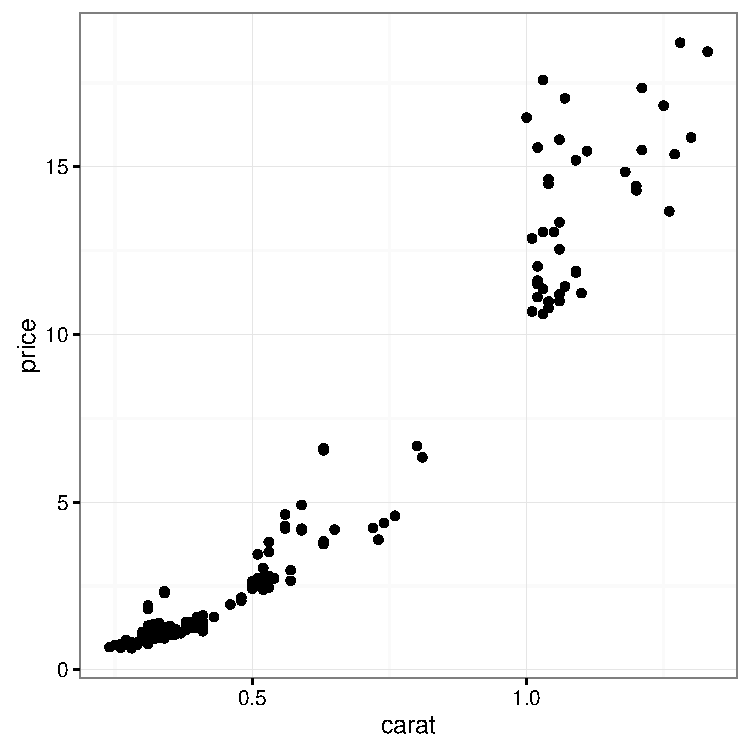
\includegraphics[width=.5\linewidth]{figure/unnamed-chunk-4-1} 

}

\caption[Plot depicting the sale price of 375 diamonds with the same quality of cut, clarity, and color]{Plot depicting the sale price of 375 diamonds with the same quality of cut, clarity, and color. There is a general pattern indicating that higher carat (i.e., the mass) is associated with higher price.}\label{fig:unnamed-chunk-4}
\end{figure}


\end{knitrout}

Here are some summaries of the data (using carat as the $x$-value and price as the $y$-value):

$$
   \sum_{i=1}^{375} x_i = 163.68 \hspace{3cm} \sum_{i=1}^{375} x_i^2 = 94.6962 \\
$$

$$
   \sum_{i=1}^{375} y_i = 1018.531 \hspace{3cm} \sum_{i=1}^{375} y_i^2 = 8802.953653 \\
$$

$$
   \sum_{i=1}^{375} x_i y_i = 808.54225
$$

\newpage

\begin{parts}
   \part
   The following parts are based on using a linear relationship between carat ($x$) and price ($y$).
   \begin{subparts}
      \subpart[5] Using the above summaries, write the equation of the fitted linear relationship between carat and price.
      \vspace{3cm}
      \subpart[3] Using the fitted line, what do we suppose the price would be for a 1.07 carat diamond?
      \vspace{3cm}
      \subpart[3] The actual price of a 1.07 carat diamond in the data is 11.434 thousand dollars. What is the residual for this specific diamond using the linear model?
      \vspace{3cm}
      \subpart[3] For the linear relationship, find $r$, the sample correlation coeffecient and $R^2$, the coeffecient of determination.
      \vspace{3cm}
      \subpart[3] Explain whether or not the fitted line did a good job describing the relationship between carat and price.
      \vspace{3cm}
   \end{subparts}

   \newpage 

   \part 
   A better fit may be found using a quadratic model, where price depends on carat and $\text{carat}^2$.
   The JMP output below comes from fitting a this quadratic relationship using price as the response (``\verb!price!") and 
   carat (\verb!carat!) and $\text{carat}^2$ (\verb!carat_sq!) as the model variables.

   \centerline{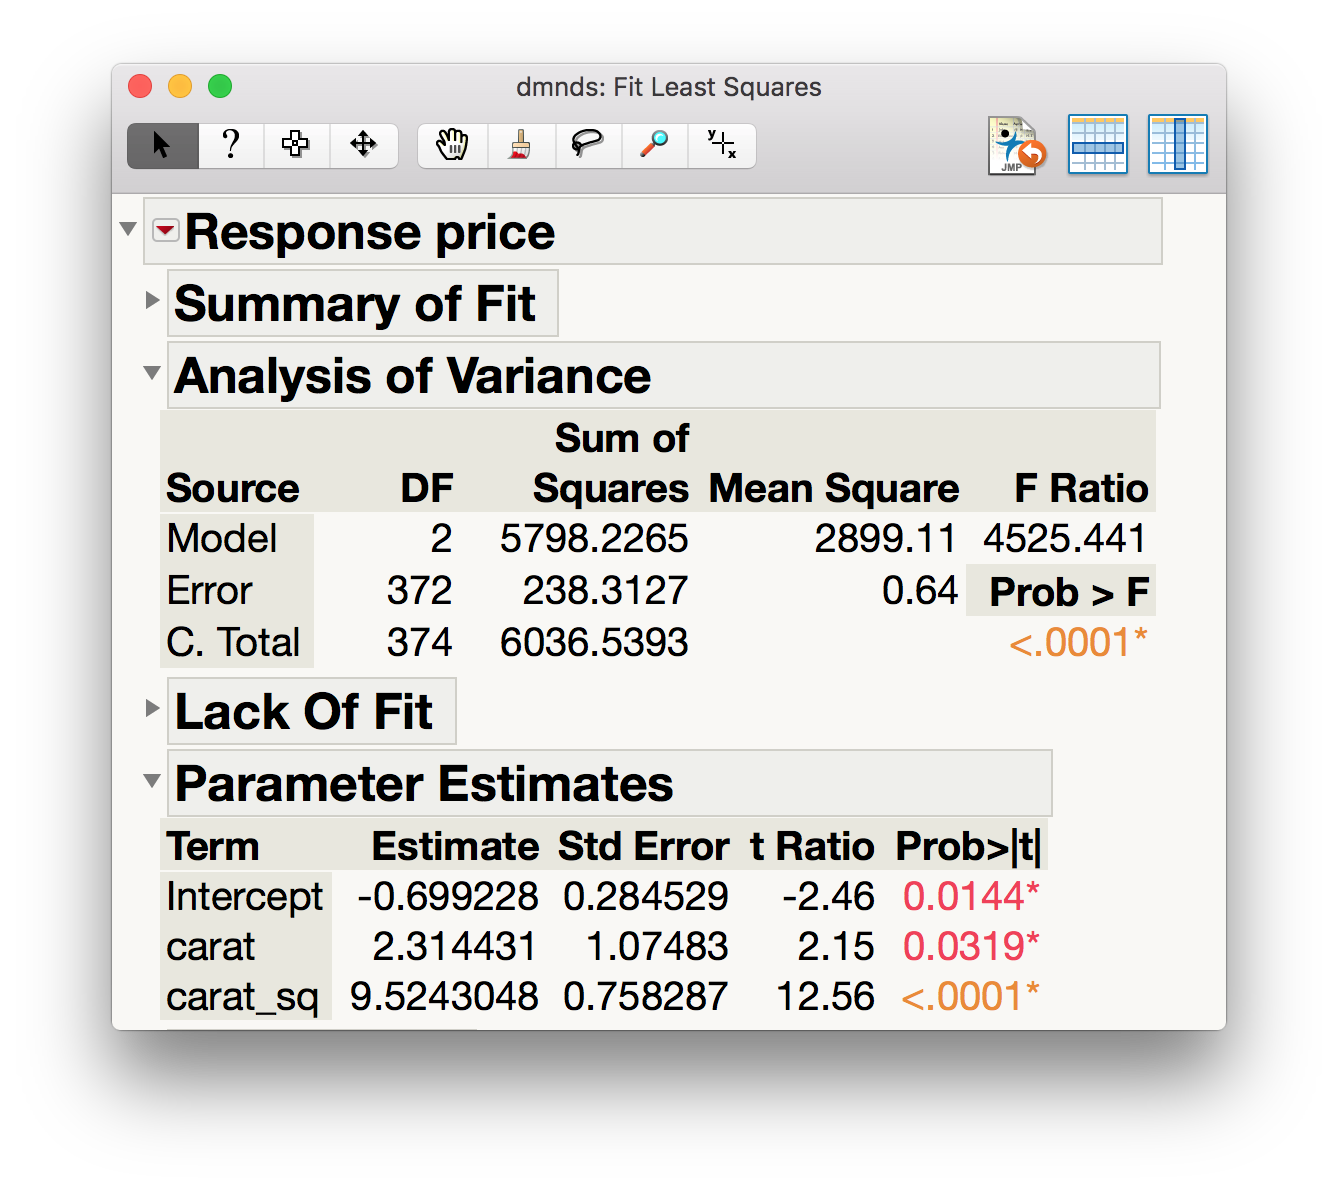
\includegraphics[scale=.35]{carat_sq_fit}}

   \begin{subparts}
      \subpart[5] Write the equation of the fitted quadratic relationship.
      \vspace{2cm}
      \subpart[3] Using the fitted quadratic relationship, what do we suppose the price would be for a 1.07 carat diamond?
      \vspace{2cm}
      \subpart[3] The actual price of a 1.07 carat diamond in the data is 11.434 thousand dollars. What is the residual for this specific diamond using the quadratic model?
      \vspace{2cm}
      \subpart[3] Find the value of $R^2$ for the fitted quadratic relationship.
      \vspace{2cm}
      \subpart[3] Does it appear that a quadratic relationship is better than the linear relationship?
      \vspace{2cm}
   \end{subparts}
\end{parts}

\newpage

\question

A furniture company conducted a study of the tensile strength of wood joints. They examined the combinations of three joint type (butt joint, overlap joint, and beveled joint) and three wood type (pine, oak, and walnut), joined by the same resin glue.
For each wood/joint-type pair, four joints were made and the stress at failure (in psi) was recorded. The results are recorded below:

%-- : R code (Code in Document)


The results are recorded below.

\begin{table}[h]
\centering
\begin{tabular}{lrrr}
   & \multicolumn{3}{c}{Joint} \\
\cline{2-4}
Wood & beveled & butt & lap \\ \hline \hline
oak     & 1688.4  & 1170.4  & 1896.5 \\
        & 1692.6  & 1164.6  & 1864.5 \\
        & 1693.9  & 1191.6  & 1855 \\
        & 1693.3  & 1186.7  & 1885.1 \\
pine    & 1226.4  & 744.3  & 1434.7 \\
        & 1234.9  & 715.4  & 1406.3 \\
        & 1247.5  & 735.4  & 1449.3 \\
        & 1220  & 734.8  & 1437.5 \\
walnut  & 1714.2  & 1216.1  & 1917.7 \\
        & 1730.5  & 1195.9  & 1897.1 \\
        & 1714.8  & 1201.3  & 1912.8 \\
        & 1724.7  & 1211.8  & 1917.2 \\
\hline
\end{tabular}
\end{table}

The following summaries may help in this problem:

%-- : R code (Code in Document)


%  \begin{table}[h]
%  \centering
%  \begin{tabular}{lrrrr}
%     & \multicolumn{3}{c}{Joint} & \\
%  \cline{2-4}
%     Wood   & beveled                                                 & butt                                                   & lap \\ \cline{1-4}\cline{1-4}
%     oak    &    $\bar{y}_{11}$ = wood_sum[1,1]               & $\bar{y}_{12}$ = wood_sum[1,2]                 & $\bar{y}_{13}$ = wood_sum[1, 3]               &  $\bar{y}_{1 \cdot}$ = woodRowMeans[1] \\
%     pine   &    $\bar{y}_{21}$ = wood_sum[2,1]               & $\bar{y}_{22}$ = wood_sum[2,2]                 & $\bar{y}_{23}$ = wood_sum[2, 3]               &  $\bar{y}_{2 \cdot}$ = woodRowMeans[2] \\
%     walnut &    $\bar{y}_{31}$ = wood_sum[3,1]               & $\bar{y}_{32}$ = wood_sum[3,2]                 & $\bar{y}_{33}$ = wood_sum[3, 3]               &  $\bar{y}_{3 \cdot}$ = woodRowMeans[3] \\
%  \cline{1-4}
%            &    $\bar{y}_{\cdot 1}$ = woodColMeans[1]        &    $\bar{y}_{\cdot 2}$ = woodColMeans[2]       & $\bar{y}_{\cdot 3}$ = woodColMeans[3]         &    $\bar{y}_{\cdot \cdot}$ = woodGrandMeans \\
%  \end{tabular}
%  \end{table}


\begin{table}[h]
\centering
\begin{tabular}{lrrrr}
   & \multicolumn{3}{c}{Joint} & \\
\cline{2-4}
   Wood   & beveled                                                 & butt                                                   & lap \\ \cline{1-4}\cline{1-4}
   oak    &    $\bar{y}_{11}$ = 1692               & $\bar{y}_{12}$ = 1178.3                 & $\bar{y}_{13}$ = 1875.3               &  $\bar{y}_{1 \cdot}$ = 1581.9 \\
   pine   &    $\bar{y}_{21}$ = 1232.2               & $\bar{y}_{22}$ = 732.5                 & $\bar{y}_{23}$ = 1432               &  $\bar{y}_{2 \cdot}$ = 1132.2 \\
   walnut &                                                         & $\bar{y}_{32}$ = 1206.3                 & $\bar{y}_{33}$ = 1911.2               &  $\bar{y}_{3 \cdot}$ = 1612.8 \\
\cline{1-4}
          &    $\bar{y}_{\cdot 1}$ = 1548.4        &                                                        & $\bar{y}_{\cdot 3}$ = 1739.5         &    $\bar{y}_{\cdot \cdot}$ = 1442.3 \\
\end{tabular}
\end{table}


\begin{parts}

   \part[2] Report the value of $\bar{y}_{31}$
   \vspace{2cm}

   \part[2] Report the value of $\bar{y}_{\cdot 2}$
   \vspace{2cm}

   \part[3] Find the fitted main effect of wood type, $a_1$, $a_2$, and $a_3$, that you would get from factorial model that ignores interactions.
   \vspace{3cm}

   \newpage

   \part[3] Ignoring possible interactions, give the estimated values $\hat{y}_{22}$ and $\hat{y}_{23}$.
   \vspace{3cm}

   \part[2] How do the estimated values computed above compare to the average for the same combinations seen in the data? 
            Does it appear that ignoring interactions was a good choice?
   \vspace{2cm}

   \part[5] Using the template below, create a profile plot for this data:

%-- : R plot (results in document)
\begin{knitrout}
\definecolor{shadecolor}{rgb}{0.969, 0.969, 0.969}\color{fgcolor}

{\centering 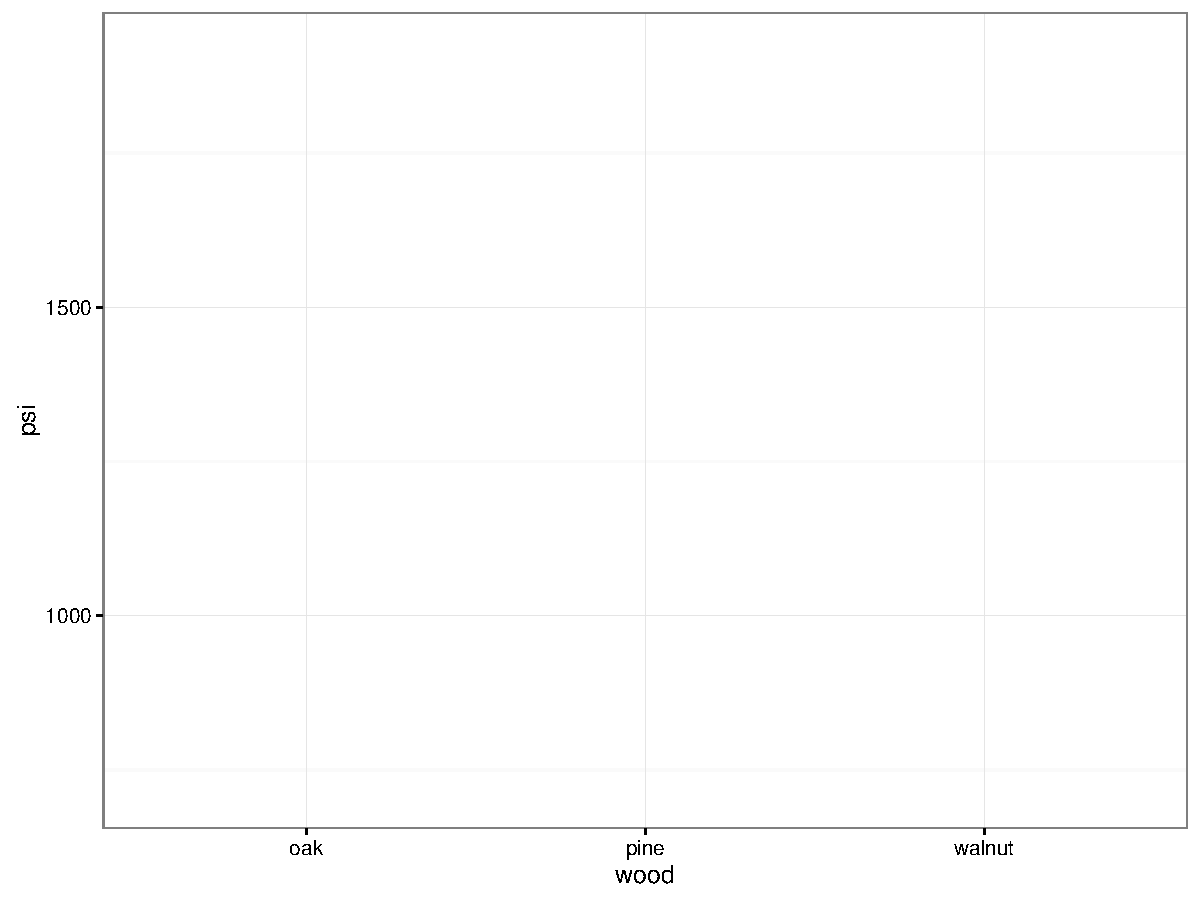
\includegraphics[width=.7\linewidth]{figure/unnamed-chunk-7-1} 

}



\end{knitrout}

   \part[2] Using the plot does it appear that there are interactions between wood type and joint type? Which combination would you recommend if we want the highest Stress at Failure?
   \vspace{2cm}
\end{parts}

\newpage
 
\question

Let $X$ be a normal random variable with a mean of 5 and a varaince of 4 (i.e., $X \sim N(5,4)$) and let $Z$ be a random variable following a standard normal distribution.
Find the following probabilities (note: the attached standard normal probability table may be helpful):
\begin{parts}
     \part[2] $P(Z \le 1.5)$

     \vspace{2cm}

     \part[2] $P(|Z| \ge 1.25)$

     \vspace{2cm}

     \part[2] $P(1 \le X < 9)$

     \vspace{2cm}

     \part[2] $P(|X| \le 5)$

     \vspace{2cm}

\end{parts}

\question 
 
 Suppose that $X$ is a continuous random variable with probability density function (pdf):
 $$
 f(x) = 
 \begin{cases}
     0 &  x < 0 \\
     2 e^{-2x} &  x \ge 0
 \end{cases}
 $$
 
 \begin{parts}
 
 \part[3] Find F(x), the cumulative probability function.
 
      \vspace{3cm}
 
 \part[3] What is the probability that $X$ takes a value less than 1?
 
      \vspace{2cm}
 
 \part[3] What is the probability that $X$ takes a value greater than 2?
 
      \vspace{2cm}
 
 \end{parts}
 
 \newpage
 
 \question
 
 Consider the following scenario:

 A fair die is rolled and the number of dots facing up is counted.
 For each dot facing up on the die, a fair coin is flipped and the number of times the coin lands heads up is recorded.
 \begin{itemize}
    \item let $N$ be the number of dots facing up from the roll of the die
    \item let $X$ be the number of heads resulting from the flips of the coin.
 \end{itemize}

 Hint: if we roll a 5 then $N = 5$ and we will toss the coin 5 times. If we consider landing on heads to be a success, then we have the conditional distribution of $X | N = 5$ to be binomial(5, $0.5$).
 More generally, we can write:
 $$
 f_{X|N}(x|n) = \frac{n!}{(n - x)! x!} (0.5)^x (0.5)^{n - x}, x = 0, 1, ..., n
 $$
 and 0 otherwise.
 
 \begin{parts}
    \part[3] Find the marginal probability function for $N$, $f_N(n)$.
    \vspace{2cm}
    \part[3] Find the conditional probability that $X = 2$ given that $N = 4$, $f_{X|N}(2|4)$.
    \vspace{2cm}
    \part[3] Find the joint probability $f_{NX}(4,2)$.
    \vspace{2cm}
    \part[3] Find the joint probability $f_{NX}(3,2)$.
    \vspace{2cm}
    \part[3] Find $f_{X}(2)$.
    \vspace{2cm}
    \part[4] Find the probability that we rolled a 4 given that we had two heads from our coin flips, $f_{N|X}(4|2)$.
    \vspace{2cm}
 \end{parts}
 
\newpage

\question

An inspector examining the dependability of a certain gas pump fills 50 containers until the pump reads 1.00 gallons. 
If the pump is completely accurate, then each container should have 1.00 gallons of gasoline.
However, since nothing is completely consistent, there will be differences from one container to the next.

Suppose that it is known that the true standard deviation of the amount of gasoline the pump recognizes as 1.00 gallons is $\sigma = 0.2$ gallons.

The average of the 50 gallon samples is $\bar{x} = 0.992$ gallons

The following table may be useful:

\begin{table}[h]
   \centering
   \caption{z's for use in Two-sided Large-$n$ intervals for the mean}
   \begin{tabular}{cc}
      \hline \\
      Desired Confidence & $z$ \\
      \hline 
      80\% & 1.28 \\
      90\% & 1.645 \\
      95\% & 1.96 \\
      98\% & 2.33 \\
      99\% & 2.58 \\
      \hline 
   \end{tabular}
\end{table}

\begin{parts}

\part[4] Provide a 90\% confidence interval for the mean volume of gasoline recognized by the pump to be 1.00 gallons.
\vspace{2cm}

\part[4] Provide a 95\% confidence interval for the mean volume of gasoline recognized by the pump to be 1.00 gallons.
\vspace{2cm}

\part[4] Provide a 99\% confidence interval for the mean volume of gasoline recognized by the pump to be 1.00 gallons.
\vspace{2cm}

\part[4] Interpret these confidence intervals - is there evidence that the meter on the pump is not accurate?

\end{parts}


% % \question
% %    After running the O-ring experiment, the researchers found $\bar{x} = 50$ K and $\bar{y} = 53$ K. 
% %    Suppose that $\sigma_X^2 = 10$ and $\sigma_Y = 20$.
% % \begin{parts}
% %    \part[4] Provide a 90\% confidence interval for $\mu_X$.
% %    \vspace{3cm}
% %    \part[4] Provide a 99\% confidence interval for $\mu_X$.
% %    \vspace{3cm}
% %    \part[4] Provide a 95\% confidence interval for $\mu_Y$.
% %    \vspace{3cm}
% %    \part[6] Provide a 95\% confidence interval for $\mu_X - \mu_Y$ (hint: you can use the distribution of $\bar{D}$). Does this provide any evidence that one O-ring is better than the other?
% %    \vspace{3cm}
% %    \part[2] Is there any evidence that one O-ring is better than the other?
% % \end{parts}
% % 
% % \newpage
% % 
% % \question
% %    
% %    A company recently did a major overhaul to their server system hardware and is checking to make sure that there have been no changes in the download speed.
% %    The previous download speed had an average of 63.4 Mbps.
% %    A systems analyst took 10 readings on the download speeds during the course of a day to check. 
% %    Her results are below (in Mbps):
% % 
% % %-- : R code (Code in Document)
% % <<echo=FALSE, cache=TRUE, include = TRUE>>=
% % 
% % dwnld_speeds <- round(rnorm(10,0,.2) + 63.4,2)
% %    
% % @
% % 
% % \begin{center}
% %    dwnld_speeds
% % \end{center}
% % 
% % The sample average is round(mean(dwnld_speeds),2) and the sample variance is round(var(dwnld_speeds),3).
% % 
% % \begin{parts}
% %    
% % 
% % \part[5] Provide a 90\% confidence interval for the mean download speed.
% % \vspace{2cm}
% % 
% % \part[5] Provide a 95\% lower confidence bound for the mean download speed.
% % \vspace{2cm}
% % 
% % \part[10] Conduct a hypothesis test at the 95\% confidence level for the null hypothesis $\mu = 63.4$ against the alternative $\mu \ne 63.4$. Include your hypothesis statement, the test statistic, the p-value, your decision rule, and your conclusion.
% % 
% % \end{parts}
% %    
 
\end{questions}
 
\end{document}
